\documentclass{beamer}


\usetheme{madrid}
\usecolortheme{beaver}
\usepackage{tikz}


\title[About Beamer]{A sample class on beamer}
\subtitle{in sleepy mode}
\author[L.M. and C.R.]{Lionel Messi \inst{1} \and Christiano Ronaldo\inst{2}}

\institute[BUET]
{
	\inst{1}
	Department of Physics\\
	BUET\\
	\inst{2}
	Department of Mathematics\\
	BUET\\
}
\date{\today}



\begin{document}
    \titlepage

   
\section{Animation}

\begin{frame}
\begin{center}
	
	\tikzset{every picture/.style={line width=0.75pt}} %set default line width to 0.75pt        
	
	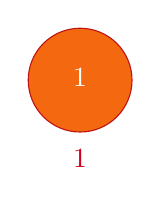
\begin{tikzpicture}[x=0.75pt,y=0.75pt,yscale=-1,xscale=1]
	%uncomment if require: \path (0,300); %set diagram left start at 0, and has height of 300
	
	\draw  [color={rgb, 255:red, 189; green, 19; blue, 19 }  ,draw opacity=1 ][fill={rgb, 255:red, 244; green, 105; blue, 16 }  ,fill opacity=1 ]  (321, 32) circle [x radius= 25, y radius= 25]  ;
	
	\draw (321,31) node [color={rgb, 255:red, 255; green, 255; blue, 255 }  ,opacity=1 ] [align=left] {1};
	\draw (321,70) node [color={rgb, 255:red, 208; green, 2; blue, 27 }  ,opacity=1 ] [align=left] {1};
	
	\end{tikzpicture} 
		
\end{center}
\end{frame}



\begin{frame}
	\begin{center}
			\tikzset{every picture/.style={line width=0.75pt}} %set default line width to 0.75pt        
		
		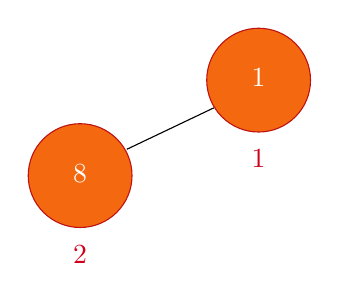
\begin{tikzpicture}[x=0.75pt,y=0.75pt,yscale=-1,xscale=1]
		%uncomment if require: \path (0,300); %set diagram left start at 0, and has height of 300
		
		\draw  [color={rgb, 255:red, 189; green, 19; blue, 19 }  ,draw opacity=1 ][fill={rgb, 255:red, 244; green, 105; blue, 16 }  ,fill opacity=1 ]  (321, 32) circle [x radius= 25, y radius= 25]  ;
		\draw  [color={rgb, 255:red, 189; green, 19; blue, 19 }  ,draw opacity=1 ][fill={rgb, 255:red, 244; green, 105; blue, 16 }  ,fill opacity=1 ]  (235, 78) circle [x radius= 25, y radius= 25]  ;
		\draw    (257.5,65.33) -- (299.5,45.33) ;
		
		
		
		\draw (321,31) node [color={rgb, 255:red, 255; green, 255; blue, 255 }  ,opacity=1 ] [align=left] {1};
		\draw (321,70) node [color={rgb, 255:red, 208; green, 2; blue, 27 }  ,opacity=1 ] [align=left] {1};
		\draw (235,77) node [color={rgb, 255:red, 255; green, 255; blue, 255 }  ,opacity=1 ] [align=left] {8};
		\draw (235,116) node [color={rgb, 255:red, 208; green, 2; blue, 27 }  ,opacity=1 ] [align=left] {2};
		
		
		\end{tikzpicture}
	\end{center}
\end{frame}



\begin{frame}
	\begin{center}
		\tikzset{every picture/.style={line width=0.75pt}} %set default line width to 0.75pt        
		
		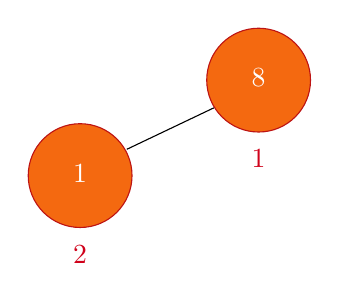
\begin{tikzpicture}[x=0.75pt,y=0.75pt,yscale=-1,xscale=1]
		%uncomment if require: \path (0,300); %set diagram left start at 0, and has height of 300
		
		\draw  [color={rgb, 255:red, 189; green, 19; blue, 19 }  ,draw opacity=1 ][fill={rgb, 255:red, 244; green, 105; blue, 16 }  ,fill opacity=1 ]  (321, 32) circle [x radius= 25, y radius= 25]  ;
		\draw  [color={rgb, 255:red, 189; green, 19; blue, 19 }  ,draw opacity=1 ][fill={rgb, 255:red, 244; green, 105; blue, 16 }  ,fill opacity=1 ]  (235, 78) circle [x radius= 25, y radius= 25]  ;
		\draw    (257.5,65.33) -- (299.5,45.33) ;
		
		
		
		\draw (321,31) node [color={rgb, 255:red, 255; green, 255; blue, 255 }  ,opacity=1 ] [align=left] {8};
		\draw (321,70) node [color={rgb, 255:red, 208; green, 2; blue, 27 }  ,opacity=1 ] [align=left] {1};
		\draw (235,77) node [color={rgb, 255:red, 255; green, 255; blue, 255 }  ,opacity=1 ] [align=left] {1};
		\draw (235,116) node [color={rgb, 255:red, 208; green, 2; blue, 27 }  ,opacity=1 ] [align=left] {2};
		
		
		\end{tikzpicture}
		
	\end{center}
\end{frame}


\begin{frame}
	\begin{center}
		\tikzset{every picture/.style={line width=0.75pt}} %set default line width to 0.75pt        
		
		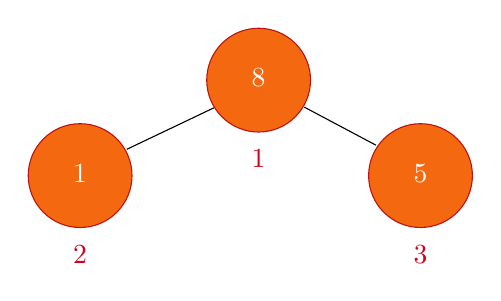
\begin{tikzpicture}[x=0.75pt,y=0.75pt,yscale=-1,xscale=1]
		%uncomment if require: \path (0,300); %set diagram left start at 0, and has height of 300
		
		\draw  [color={rgb, 255:red, 189; green, 19; blue, 19 }  ,draw opacity=1 ][fill={rgb, 255:red, 244; green, 105; blue, 16 }  ,fill opacity=1 ]  (321, 32) circle [x radius= 25, y radius= 25]  ;
		\draw  [color={rgb, 255:red, 189; green, 19; blue, 19 }  ,draw opacity=1 ][fill={rgb, 255:red, 244; green, 105; blue, 16 }  ,fill opacity=1 ]  (235, 78) circle [x radius= 25, y radius= 25]  ;
		\draw    (257.5,65.33) -- (299.5,45.33) ;
		
		
		\draw  [color={rgb, 255:red, 189; green, 19; blue, 19 }  ,draw opacity=1 ][fill={rgb, 255:red, 244; green, 105; blue, 16 }  ,fill opacity=1 ]  (399, 78) circle [x radius= 25, y radius= 25]  ;
		\draw    (343,45) -- (377.5,63.33) ;
		
		
		
		\draw (321,31) node [color={rgb, 255:red, 255; green, 255; blue, 255 }  ,opacity=1 ] [align=left] {8};
		\draw (321,70) node [color={rgb, 255:red, 208; green, 2; blue, 27 }  ,opacity=1 ] [align=left] {1};
		\draw (235,77) node [color={rgb, 255:red, 255; green, 255; blue, 255 }  ,opacity=1 ] [align=left] {1};
		\draw (235,116) node [color={rgb, 255:red, 208; green, 2; blue, 27 }  ,opacity=1 ] [align=left] {2};
		\draw (399,77) node [color={rgb, 255:red, 255; green, 255; blue, 255 }  ,opacity=1 ] [align=left] {5};
		\draw (399,116) node [color={rgb, 255:red, 208; green, 2; blue, 27 }  ,opacity=1 ] [align=left] {3};
		
		
		\end{tikzpicture}
		
	\end{center}
\end{frame}


\begin{frame}
	\begin{center}
		\tikzset{every picture/.style={line width=0.75pt}} %set default line width to 0.75pt        
		
		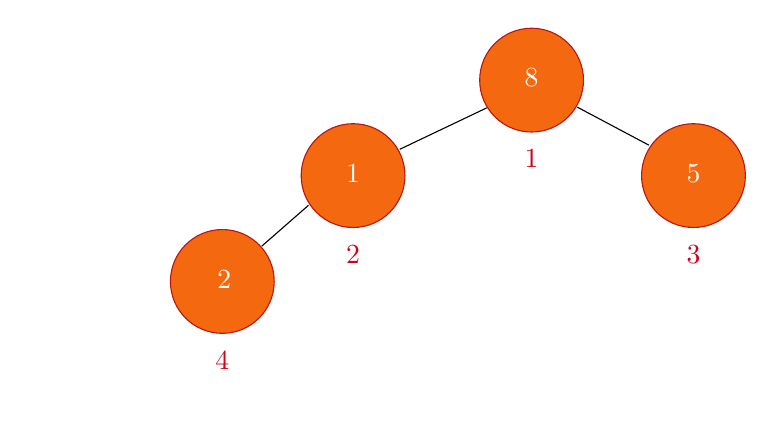
\begin{tikzpicture}[x=0.75pt,y=0.75pt,yscale=-1,xscale=1]
		%uncomment if require: \path (0,300); %set diagram left start at 0, and has height of 300
		
		\draw  [color={rgb, 255:red, 189; green, 19; blue, 19 }  ,draw opacity=1 ][fill={rgb, 255:red, 244; green, 105; blue, 16 }  ,fill opacity=1 ]  (321, 32) circle [x radius= 25, y radius= 25]  ;
		\draw  [color={rgb, 255:red, 189; green, 19; blue, 19 }  ,draw opacity=1 ][fill={rgb, 255:red, 244; green, 105; blue, 16 }  ,fill opacity=1 ]  (235, 78) circle [x radius= 25, y radius= 25]  ;
		\draw    (257.5,65.33) -- (299.5,45.33) ;
		
		
		\draw  [color={rgb, 255:red, 189; green, 19; blue, 19 }  ,draw opacity=1 ][fill={rgb, 255:red, 244; green, 105; blue, 16 }  ,fill opacity=1 ]  (399, 78) circle [x radius= 25, y radius= 25]  ;
		\draw    (343,45) -- (377.5,63.33) ;
		
		
		\draw  [color={rgb, 255:red, 189; green, 19; blue, 19 }  ,draw opacity=1 ][fill={rgb, 255:red, 244; green, 105; blue, 16 }  ,fill opacity=1 ]  (172, 129) circle [x radius= 25, y radius= 25]  ;
		\draw    (191,112) -- (213.5,92.33) ;
		
		
		
		\draw (321,31) node [color={rgb, 255:red, 255; green, 255; blue, 255 }  ,opacity=1 ] [align=left] {8};
		\draw (321,70) node [color={rgb, 255:red, 208; green, 2; blue, 27 }  ,opacity=1 ] [align=left] {1};
		\draw (235,77) node [color={rgb, 255:red, 255; green, 255; blue, 255 }  ,opacity=1 ] [align=left] {1};
		\draw (235,116) node [color={rgb, 255:red, 208; green, 2; blue, 27 }  ,opacity=1 ] [align=left] {2};
		\draw (399,77) node [color={rgb, 255:red, 255; green, 255; blue, 255 }  ,opacity=1 ] [align=left] {5};
		\draw (399,116) node [color={rgb, 255:red, 208; green, 2; blue, 27 }  ,opacity=1 ] [align=left] {3};
		\draw (173,128) node [color={rgb, 255:red, 255; green, 255; blue, 255 }  ,opacity=1 ] [align=left] {2};
		\draw (172,167) node [color={rgb, 255:red, 208; green, 2; blue, 27 }  ,opacity=1 ] [align=left] {4};
		\draw (86,174) node [color={rgb, 255:red, 255; green, 255; blue, 255 }  ,opacity=1 ] [align=left] {1};
		\draw (250,174) node [color={rgb, 255:red, 255; green, 255; blue, 255 }  ,opacity=1 ] [align=left] {5};
		
		
		\end{tikzpicture}
	\end{center}
\end{frame}


\begin{frame}
	\begin{center}
			\tikzset{every picture/.style={line width=0.75pt}} %set default line width to 0.75pt        
		
		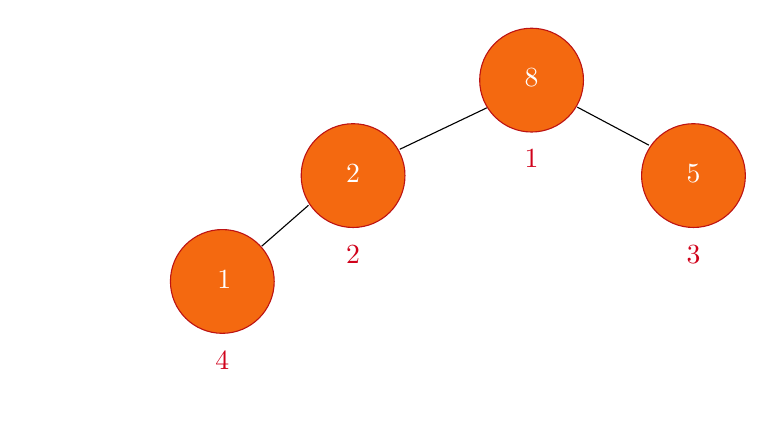
\begin{tikzpicture}[x=0.75pt,y=0.75pt,yscale=-1,xscale=1]
		%uncomment if require: \path (0,300); %set diagram left start at 0, and has height of 300
		
		\draw  [color={rgb, 255:red, 189; green, 19; blue, 19 }  ,draw opacity=1 ][fill={rgb, 255:red, 244; green, 105; blue, 16 }  ,fill opacity=1 ]  (321, 32) circle [x radius= 25, y radius= 25]  ;
		\draw  [color={rgb, 255:red, 189; green, 19; blue, 19 }  ,draw opacity=1 ][fill={rgb, 255:red, 244; green, 105; blue, 16 }  ,fill opacity=1 ]  (235, 78) circle [x radius= 25, y radius= 25]  ;
		\draw    (257.5,65.33) -- (299.5,45.33) ;
		
		
		\draw  [color={rgb, 255:red, 189; green, 19; blue, 19 }  ,draw opacity=1 ][fill={rgb, 255:red, 244; green, 105; blue, 16 }  ,fill opacity=1 ]  (399, 78) circle [x radius= 25, y radius= 25]  ;
		\draw    (343,45) -- (377.5,63.33) ;
		
		
		\draw  [color={rgb, 255:red, 189; green, 19; blue, 19 }  ,draw opacity=1 ][fill={rgb, 255:red, 244; green, 105; blue, 16 }  ,fill opacity=1 ]  (172, 129) circle [x radius= 25, y radius= 25]  ;
		\draw    (191,112) -- (213.5,92.33) ;
		
		
		
		\draw (321,31) node [color={rgb, 255:red, 255; green, 255; blue, 255 }  ,opacity=1 ] [align=left] {8};
		\draw (321,70) node [color={rgb, 255:red, 208; green, 2; blue, 27 }  ,opacity=1 ] [align=left] {1};
		\draw (235,77) node [color={rgb, 255:red, 255; green, 255; blue, 255 }  ,opacity=1 ] [align=left] {2};
		\draw (235,116) node [color={rgb, 255:red, 208; green, 2; blue, 27 }  ,opacity=1 ] [align=left] {2};
		\draw (399,77) node [color={rgb, 255:red, 255; green, 255; blue, 255 }  ,opacity=1 ] [align=left] {5};
		\draw (399,116) node [color={rgb, 255:red, 208; green, 2; blue, 27 }  ,opacity=1 ] [align=left] {3};
		\draw (173,128) node [color={rgb, 255:red, 255; green, 255; blue, 255 }  ,opacity=1 ] [align=left] {1};
		\draw (172,167) node [color={rgb, 255:red, 208; green, 2; blue, 27 }  ,opacity=1 ] [align=left] {4};
		\draw (86,174) node [color={rgb, 255:red, 255; green, 255; blue, 255 }  ,opacity=1 ] [align=left] {1};
		\draw (250,174) node [color={rgb, 255:red, 255; green, 255; blue, 255 }  ,opacity=1 ] [align=left] {5};
		
		
		\end{tikzpicture}
	\end{center}
\end{frame}

\begin{frame}
   \begin{center}
   	\tikzset{every picture/.style={line width=0.75pt}} %set default line width to 0.75pt        
   	
   	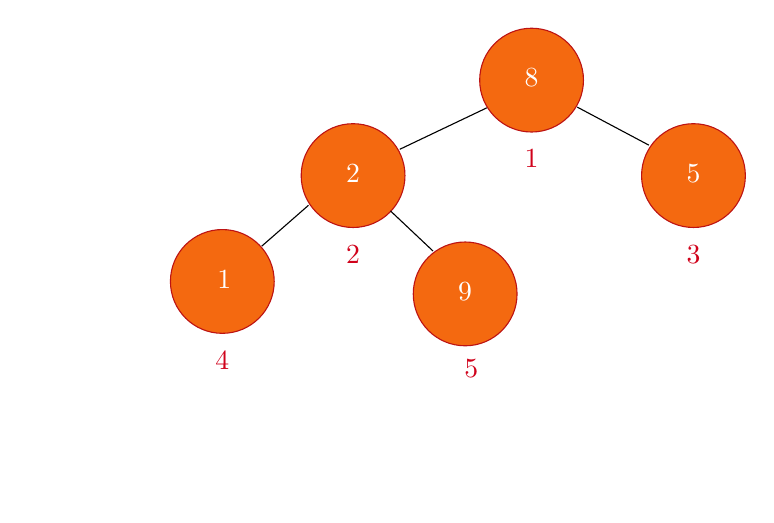
\begin{tikzpicture}[x=0.75pt,y=0.75pt,yscale=-1,xscale=1]
   	%uncomment if require: \path (0,300); %set diagram left start at 0, and has height of 300
   	
   	\draw  [color={rgb, 255:red, 189; green, 19; blue, 19 }  ,draw opacity=1 ][fill={rgb, 255:red, 244; green, 105; blue, 16 }  ,fill opacity=1 ]  (321, 32) circle [x radius= 25, y radius= 25]  ;
   	\draw  [color={rgb, 255:red, 189; green, 19; blue, 19 }  ,draw opacity=1 ][fill={rgb, 255:red, 244; green, 105; blue, 16 }  ,fill opacity=1 ]  (235, 78) circle [x radius= 25, y radius= 25]  ;
   	\draw    (257.5,65.33) -- (299.5,45.33) ;
   	
   	
   	\draw  [color={rgb, 255:red, 189; green, 19; blue, 19 }  ,draw opacity=1 ][fill={rgb, 255:red, 244; green, 105; blue, 16 }  ,fill opacity=1 ]  (399, 78) circle [x radius= 25, y radius= 25]  ;
   	\draw    (343,45) -- (377.5,63.33) ;
   	
   	
   	\draw  [color={rgb, 255:red, 189; green, 19; blue, 19 }  ,draw opacity=1 ][fill={rgb, 255:red, 244; green, 105; blue, 16 }  ,fill opacity=1 ]  (172, 129) circle [x radius= 25, y radius= 25]  ;
   	\draw    (191,112) -- (213.5,92.33) ;
   	
   	
   	\draw  [color={rgb, 255:red, 189; green, 19; blue, 19 }  ,draw opacity=1 ][fill={rgb, 255:red, 244; green, 105; blue, 16 }  ,fill opacity=1 ]  (289, 135) circle [x radius= 25, y radius= 25]  ;
   	\draw    (253,95) -- (273.5,114.33) ;
   	
   	
   	
   	\draw (321,31) node [color={rgb, 255:red, 255; green, 255; blue, 255 }  ,opacity=1 ] [align=left] {8};
   	\draw (321,70) node [color={rgb, 255:red, 208; green, 2; blue, 27 }  ,opacity=1 ] [align=left] {1};
   	\draw (235,77) node [color={rgb, 255:red, 255; green, 255; blue, 255 }  ,opacity=1 ] [align=left] {2};
   	\draw (235,116) node [color={rgb, 255:red, 208; green, 2; blue, 27 }  ,opacity=1 ] [align=left] {2};
   	\draw (399,77) node [color={rgb, 255:red, 255; green, 255; blue, 255 }  ,opacity=1 ] [align=left] {5};
   	\draw (399,116) node [color={rgb, 255:red, 208; green, 2; blue, 27 }  ,opacity=1 ] [align=left] {3};
   	\draw (173,128) node [color={rgb, 255:red, 255; green, 255; blue, 255 }  ,opacity=1 ] [align=left] {1};
   	\draw (172,167) node [color={rgb, 255:red, 208; green, 2; blue, 27 }  ,opacity=1 ] [align=left] {4};
   	\draw (86,174) node [color={rgb, 255:red, 255; green, 255; blue, 255 }  ,opacity=1 ] [align=left] {1};
   	\draw (250,174) node [color={rgb, 255:red, 255; green, 255; blue, 255 }  ,opacity=1 ] [align=left] {5};
   	\draw (289,134) node [color={rgb, 255:red, 255; green, 255; blue, 255 }  ,opacity=1 ] [align=left] {9};
   	\draw (292,171) node [color={rgb, 255:red, 208; green, 2; blue, 27 }  ,opacity=1 ] [align=left] {5};
   	\draw (304,223) node [color={rgb, 255:red, 255; green, 255; blue, 255 }  ,opacity=1 ] [align=left] {5};
   	
   	
   	\end{tikzpicture}
   \end{center}
\end{frame}


\begin{frame}
	\begin{center}
		\tikzset{every picture/.style={line width=0.75pt}} %set default line width to 0.75pt        
		
		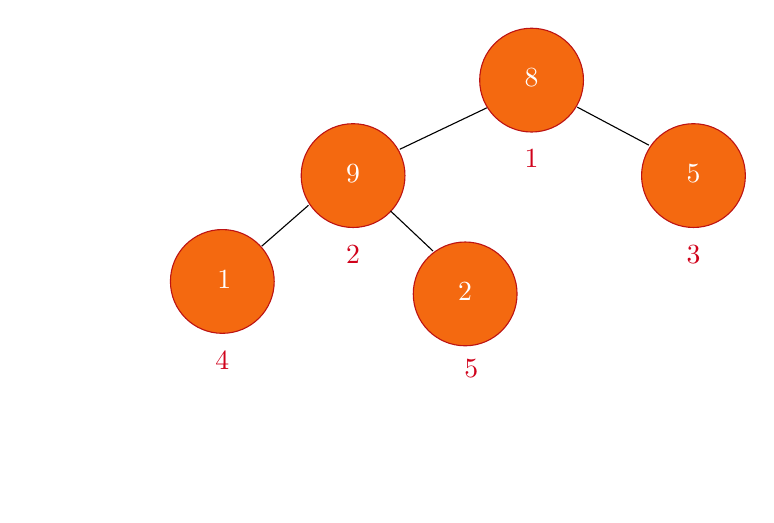
\begin{tikzpicture}[x=0.75pt,y=0.75pt,yscale=-1,xscale=1]
		%uncomment if require: \path (0,300); %set diagram left start at 0, and has height of 300
		
		\draw  [color={rgb, 255:red, 189; green, 19; blue, 19 }  ,draw opacity=1 ][fill={rgb, 255:red, 244; green, 105; blue, 16 }  ,fill opacity=1 ]  (321, 32) circle [x radius= 25, y radius= 25]  ;
		\draw  [color={rgb, 255:red, 189; green, 19; blue, 19 }  ,draw opacity=1 ][fill={rgb, 255:red, 244; green, 105; blue, 16 }  ,fill opacity=1 ]  (235, 78) circle [x radius= 25, y radius= 25]  ;
		\draw    (257.5,65.33) -- (299.5,45.33) ;
		
		
		\draw  [color={rgb, 255:red, 189; green, 19; blue, 19 }  ,draw opacity=1 ][fill={rgb, 255:red, 244; green, 105; blue, 16 }  ,fill opacity=1 ]  (399, 78) circle [x radius= 25, y radius= 25]  ;
		\draw    (343,45) -- (377.5,63.33) ;
		
		
		\draw  [color={rgb, 255:red, 189; green, 19; blue, 19 }  ,draw opacity=1 ][fill={rgb, 255:red, 244; green, 105; blue, 16 }  ,fill opacity=1 ]  (172, 129) circle [x radius= 25, y radius= 25]  ;
		\draw    (191,112) -- (213.5,92.33) ;
		
		
		\draw  [color={rgb, 255:red, 189; green, 19; blue, 19 }  ,draw opacity=1 ][fill={rgb, 255:red, 244; green, 105; blue, 16 }  ,fill opacity=1 ]  (289, 135) circle [x radius= 25, y radius= 25]  ;
		\draw    (253,95) -- (273.5,114.33) ;
		
		
		
		\draw (321,31) node [color={rgb, 255:red, 255; green, 255; blue, 255 }  ,opacity=1 ] [align=left] {8};
		\draw (321,70) node [color={rgb, 255:red, 208; green, 2; blue, 27 }  ,opacity=1 ] [align=left] {1};
		\draw (235,77) node [color={rgb, 255:red, 255; green, 255; blue, 255 }  ,opacity=1 ] [align=left] {9};
		\draw (235,116) node [color={rgb, 255:red, 208; green, 2; blue, 27 }  ,opacity=1 ] [align=left] {2};
		\draw (399,77) node [color={rgb, 255:red, 255; green, 255; blue, 255 }  ,opacity=1 ] [align=left] {5};
		\draw (399,116) node [color={rgb, 255:red, 208; green, 2; blue, 27 }  ,opacity=1 ] [align=left] {3};
		\draw (173,128) node [color={rgb, 255:red, 255; green, 255; blue, 255 }  ,opacity=1 ] [align=left] {1};
		\draw (172,167) node [color={rgb, 255:red, 208; green, 2; blue, 27 }  ,opacity=1 ] [align=left] {4};
		\draw (86,174) node [color={rgb, 255:red, 255; green, 255; blue, 255 }  ,opacity=1 ] [align=left] {1};
		\draw (250,174) node [color={rgb, 255:red, 255; green, 255; blue, 255 }  ,opacity=1 ] [align=left] {5};
		\draw (289,134) node [color={rgb, 255:red, 255; green, 255; blue, 255 }  ,opacity=1 ] [align=left] {2};
		\draw (292,171) node [color={rgb, 255:red, 208; green, 2; blue, 27 }  ,opacity=1 ] [align=left] {5};
		\draw (304,223) node [color={rgb, 255:red, 255; green, 255; blue, 255 }  ,opacity=1 ] [align=left] {5};
		
		\end{tikzpicture}
	\end{center}
\end{frame}


\begin{frame}
     \begin{center}
     	\tikzset{every picture/.style={line width=0.75pt}} %set default line width to 0.75pt        
     	
     	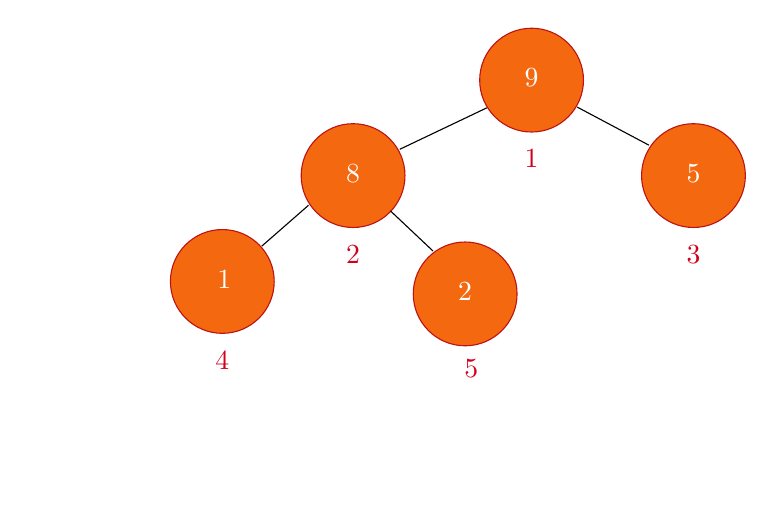
\begin{tikzpicture}[x=0.75pt,y=0.75pt,yscale=-1,xscale=1]
     	%uncomment if require: \path (0,300); %set diagram left start at 0, and has height of 300
     	
     	\draw  [color={rgb, 255:red, 189; green, 19; blue, 19 }  ,draw opacity=1 ][fill={rgb, 255:red, 244; green, 105; blue, 16 }  ,fill opacity=1 ]  (321, 32) circle [x radius= 25, y radius= 25]  ;
     	\draw  [color={rgb, 255:red, 189; green, 19; blue, 19 }  ,draw opacity=1 ][fill={rgb, 255:red, 244; green, 105; blue, 16 }  ,fill opacity=1 ]  (235, 78) circle [x radius= 25, y radius= 25]  ;
     	\draw    (257.5,65.33) -- (299.5,45.33) ;
     	
     	
     	\draw  [color={rgb, 255:red, 189; green, 19; blue, 19 }  ,draw opacity=1 ][fill={rgb, 255:red, 244; green, 105; blue, 16 }  ,fill opacity=1 ]  (399, 78) circle [x radius= 25, y radius= 25]  ;
     	\draw    (343,45) -- (377.5,63.33) ;
     	
     	
     	\draw  [color={rgb, 255:red, 189; green, 19; blue, 19 }  ,draw opacity=1 ][fill={rgb, 255:red, 244; green, 105; blue, 16 }  ,fill opacity=1 ]  (172, 129) circle [x radius= 25, y radius= 25]  ;
     	\draw    (191,112) -- (213.5,92.33) ;
     	
     	
     	\draw  [color={rgb, 255:red, 189; green, 19; blue, 19 }  ,draw opacity=1 ][fill={rgb, 255:red, 244; green, 105; blue, 16 }  ,fill opacity=1 ]  (289, 135) circle [x radius= 25, y radius= 25]  ;
     	\draw    (253,95) -- (273.5,114.33) ;
     	
     	
     	
     	\draw (321,31) node [color={rgb, 255:red, 255; green, 255; blue, 255 }  ,opacity=1 ] [align=left] {9};
     	\draw (321,70) node [color={rgb, 255:red, 208; green, 2; blue, 27 }  ,opacity=1 ] [align=left] {1};
     	\draw (235,77) node [color={rgb, 255:red, 255; green, 255; blue, 255 }  ,opacity=1 ] [align=left] {8};
     	\draw (235,116) node [color={rgb, 255:red, 208; green, 2; blue, 27 }  ,opacity=1 ] [align=left] {2};
     	\draw (399,77) node [color={rgb, 255:red, 255; green, 255; blue, 255 }  ,opacity=1 ] [align=left] {5};
     	\draw (399,116) node [color={rgb, 255:red, 208; green, 2; blue, 27 }  ,opacity=1 ] [align=left] {3};
     	\draw (173,128) node [color={rgb, 255:red, 255; green, 255; blue, 255 }  ,opacity=1 ] [align=left] {1};
     	\draw (172,167) node [color={rgb, 255:red, 208; green, 2; blue, 27 }  ,opacity=1 ] [align=left] {4};
     	\draw (86,174) node [color={rgb, 255:red, 255; green, 255; blue, 255 }  ,opacity=1 ] [align=left] {1};
     	\draw (250,174) node [color={rgb, 255:red, 255; green, 255; blue, 255 }  ,opacity=1 ] [align=left] {5};
     	\draw (289,134) node [color={rgb, 255:red, 255; green, 255; blue, 255 }  ,opacity=1 ] [align=left] {2};
     	\draw (292,171) node [color={rgb, 255:red, 208; green, 2; blue, 27 }  ,opacity=1 ] [align=left] {5};
     	\draw (304,223) node [color={rgb, 255:red, 255; green, 255; blue, 255 }  ,opacity=1 ] [align=left] {5};
     	
     	
     	\end{tikzpicture}
     \end{center}
\end{frame}

\begin{frame}
	\begin{center}
		\tikzset{every picture/.style={line width=0.75pt}} %set default line width to 0.75pt        
		
		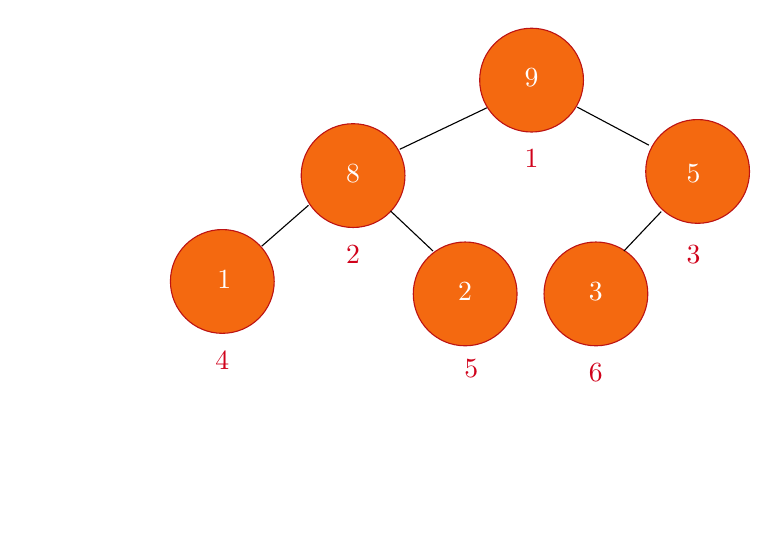
\begin{tikzpicture}[x=0.75pt,y=0.75pt,yscale=-1,xscale=1]
		%uncomment if require: \path (0,300); %set diagram left start at 0, and has height of 300
		
		\draw  [color={rgb, 255:red, 189; green, 19; blue, 19 }  ,draw opacity=1 ][fill={rgb, 255:red, 244; green, 105; blue, 16 }  ,fill opacity=1 ]  (321, 32) circle [x radius= 25, y radius= 25]  ;
		\draw  [color={rgb, 255:red, 189; green, 19; blue, 19 }  ,draw opacity=1 ][fill={rgb, 255:red, 244; green, 105; blue, 16 }  ,fill opacity=1 ]  (235, 78) circle [x radius= 25, y radius= 25]  ;
		\draw    (257.5,65.33) -- (299.5,45.33) ;
		
		
		\draw  [color={rgb, 255:red, 189; green, 19; blue, 19 }  ,draw opacity=1 ][fill={rgb, 255:red, 244; green, 105; blue, 16 }  ,fill opacity=1 ]  (401, 76) circle [x radius= 25, y radius= 25]  ;
		\draw    (343,45) -- (377.5,63.33) ;
		
		
		\draw  [color={rgb, 255:red, 189; green, 19; blue, 19 }  ,draw opacity=1 ][fill={rgb, 255:red, 244; green, 105; blue, 16 }  ,fill opacity=1 ]  (172, 129) circle [x radius= 25, y radius= 25]  ;
		\draw    (191,112) -- (213.5,92.33) ;
		
		
		\draw  [color={rgb, 255:red, 189; green, 19; blue, 19 }  ,draw opacity=1 ][fill={rgb, 255:red, 244; green, 105; blue, 16 }  ,fill opacity=1 ]  (289, 135) circle [x radius= 25, y radius= 25]  ;
		\draw    (253,95) -- (273.5,114.33) ;
		
		
		\draw  [color={rgb, 255:red, 189; green, 19; blue, 19 }  ,draw opacity=1 ][fill={rgb, 255:red, 244; green, 105; blue, 16 }  ,fill opacity=1 ]  (352, 135) circle [x radius= 25, y radius= 25]  ;
		\draw    (365.5,114.33) -- (383.5,95.33) ;
		
		
		
		\draw (321,31) node [color={rgb, 255:red, 255; green, 255; blue, 255 }  ,opacity=1 ] [align=left] {9};
		\draw (321,70) node [color={rgb, 255:red, 208; green, 2; blue, 27 }  ,opacity=1 ] [align=left] {1};
		\draw (235,77) node [color={rgb, 255:red, 255; green, 255; blue, 255 }  ,opacity=1 ] [align=left] {8};
		\draw (235,116) node [color={rgb, 255:red, 208; green, 2; blue, 27 }  ,opacity=1 ] [align=left] {2};
		\draw (399,77) node [color={rgb, 255:red, 255; green, 255; blue, 255 }  ,opacity=1 ] [align=left] {5};
		\draw (399,116) node [color={rgb, 255:red, 208; green, 2; blue, 27 }  ,opacity=1 ] [align=left] {3};
		\draw (173,128) node [color={rgb, 255:red, 255; green, 255; blue, 255 }  ,opacity=1 ] [align=left] {1};
		\draw (172,167) node [color={rgb, 255:red, 208; green, 2; blue, 27 }  ,opacity=1 ] [align=left] {4};
		\draw (86,174) node [color={rgb, 255:red, 255; green, 255; blue, 255 }  ,opacity=1 ] [align=left] {1};
		\draw (250,174) node [color={rgb, 255:red, 255; green, 255; blue, 255 }  ,opacity=1 ] [align=left] {5};
		\draw (289,134) node [color={rgb, 255:red, 255; green, 255; blue, 255 }  ,opacity=1 ] [align=left] {2};
		\draw (292,171) node [color={rgb, 255:red, 208; green, 2; blue, 27 }  ,opacity=1 ] [align=left] {5};
		\draw (352,134) node [color={rgb, 255:red, 255; green, 255; blue, 255 }  ,opacity=1 ] [align=left] {3};
		\draw (352,173) node [color={rgb, 255:red, 208; green, 2; blue, 27 }  ,opacity=1 ] [align=left] {6};
		\draw (290,185) node [color={rgb, 255:red, 255; green, 255; blue, 255 }  ,opacity=1 ] [align=left] {1};
		\draw (367,231) node [color={rgb, 255:red, 255; green, 255; blue, 255 }  ,opacity=1 ] [align=left] {5};
		
		
		\end{tikzpicture}
	\end{center}
\end{frame}


\begin{frame}
	\begin{center}
		\tikzset{every picture/.style={line width=0.75pt}} %set default line width to 0.75pt        
		
		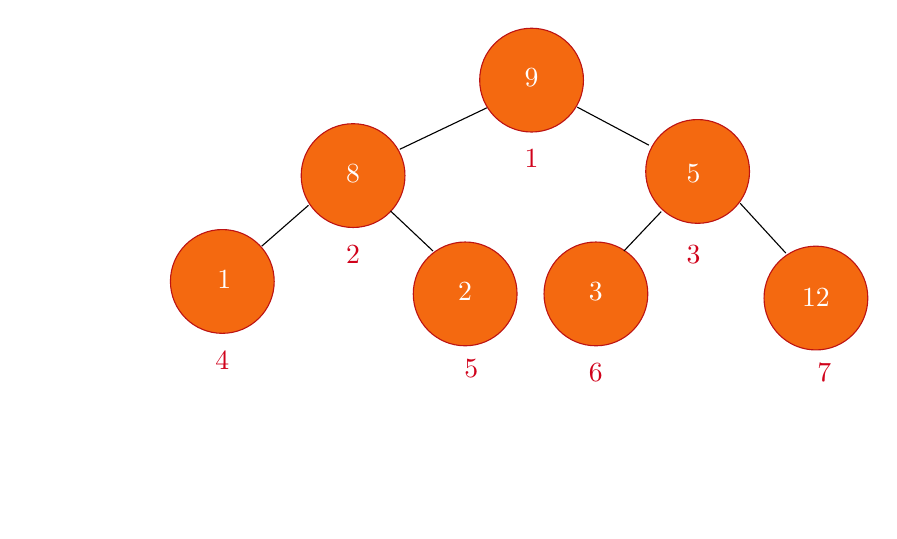
\begin{tikzpicture}[x=0.75pt,y=0.75pt,yscale=-1,xscale=1]
		%uncomment if require: \path (0,300); %set diagram left start at 0, and has height of 300
		
		\draw  [color={rgb, 255:red, 189; green, 19; blue, 19 }  ,draw opacity=1 ][fill={rgb, 255:red, 244; green, 105; blue, 16 }  ,fill opacity=1 ]  (321, 32) circle [x radius= 25, y radius= 25]  ;
		\draw  [color={rgb, 255:red, 189; green, 19; blue, 19 }  ,draw opacity=1 ][fill={rgb, 255:red, 244; green, 105; blue, 16 }  ,fill opacity=1 ]  (235, 78) circle [x radius= 25, y radius= 25]  ;
		\draw    (257.5,65.33) -- (299.5,45.33) ;
		
		
		\draw  [color={rgb, 255:red, 189; green, 19; blue, 19 }  ,draw opacity=1 ][fill={rgb, 255:red, 244; green, 105; blue, 16 }  ,fill opacity=1 ]  (401, 76) circle [x radius= 25, y radius= 25]  ;
		\draw    (343,45) -- (377.5,63.33) ;
		
		
		\draw  [color={rgb, 255:red, 189; green, 19; blue, 19 }  ,draw opacity=1 ][fill={rgb, 255:red, 244; green, 105; blue, 16 }  ,fill opacity=1 ]  (172, 129) circle [x radius= 25, y radius= 25]  ;
		\draw    (191,112) -- (213.5,92.33) ;
		
		
		\draw  [color={rgb, 255:red, 189; green, 19; blue, 19 }  ,draw opacity=1 ][fill={rgb, 255:red, 244; green, 105; blue, 16 }  ,fill opacity=1 ]  (289, 135) circle [x radius= 25, y radius= 25]  ;
		\draw    (253,95) -- (273.5,114.33) ;
		
		
		\draw  [color={rgb, 255:red, 189; green, 19; blue, 19 }  ,draw opacity=1 ][fill={rgb, 255:red, 244; green, 105; blue, 16 }  ,fill opacity=1 ]  (352, 135) circle [x radius= 25, y radius= 25]  ;
		\draw    (365.5,114.33) -- (383.5,95.33) ;
		
		
		\draw  [color={rgb, 255:red, 189; green, 19; blue, 19 }  ,draw opacity=1 ][fill={rgb, 255:red, 244; green, 105; blue, 16 }  ,fill opacity=1 ]  (458, 137) circle [x radius= 25, y radius= 25]  ;
		\draw    (421.5,91.33) -- (443.5,115.33) ;
		
		
		
		\draw (321,31) node [color={rgb, 255:red, 255; green, 255; blue, 255 }  ,opacity=1 ] [align=left] {9};
		\draw (321,70) node [color={rgb, 255:red, 208; green, 2; blue, 27 }  ,opacity=1 ] [align=left] {1};
		\draw (235,77) node [color={rgb, 255:red, 255; green, 255; blue, 255 }  ,opacity=1 ] [align=left] {8};
		\draw (235,116) node [color={rgb, 255:red, 208; green, 2; blue, 27 }  ,opacity=1 ] [align=left] {2};
		\draw (399,77) node [color={rgb, 255:red, 255; green, 255; blue, 255 }  ,opacity=1 ] [align=left] {5};
		\draw (399,116) node [color={rgb, 255:red, 208; green, 2; blue, 27 }  ,opacity=1 ] [align=left] {3};
		\draw (173,128) node [color={rgb, 255:red, 255; green, 255; blue, 255 }  ,opacity=1 ] [align=left] {1};
		\draw (172,167) node [color={rgb, 255:red, 208; green, 2; blue, 27 }  ,opacity=1 ] [align=left] {4};
		\draw (86,174) node [color={rgb, 255:red, 255; green, 255; blue, 255 }  ,opacity=1 ] [align=left] {1};
		\draw (250,174) node [color={rgb, 255:red, 255; green, 255; blue, 255 }  ,opacity=1 ] [align=left] {5};
		\draw (289,134) node [color={rgb, 255:red, 255; green, 255; blue, 255 }  ,opacity=1 ] [align=left] {2};
		\draw (292,171) node [color={rgb, 255:red, 208; green, 2; blue, 27 }  ,opacity=1 ] [align=left] {5};
		\draw (352,134) node [color={rgb, 255:red, 255; green, 255; blue, 255 }  ,opacity=1 ] [align=left] {3};
		\draw (352,173) node [color={rgb, 255:red, 208; green, 2; blue, 27 }  ,opacity=1 ] [align=left] {6};
		\draw (290,185) node [color={rgb, 255:red, 255; green, 255; blue, 255 }  ,opacity=1 ] [align=left] {1};
		\draw (367,231) node [color={rgb, 255:red, 255; green, 255; blue, 255 }  ,opacity=1 ] [align=left] {5};
		\draw (458,137) node [color={rgb, 255:red, 255; green, 255; blue, 255 }  ,opacity=1 ] [align=left] {12};
		\draw (462,173) node [color={rgb, 255:red, 208; green, 2; blue, 27 }  ,opacity=1 ] [align=left] {7};
		
		
		\end{tikzpicture}
	\end{center}
\end{frame}

\begin{frame}
    \begin{center}
    	\tikzset{every picture/.style={line width=0.75pt}} %set default line width to 0.75pt        
    	
    	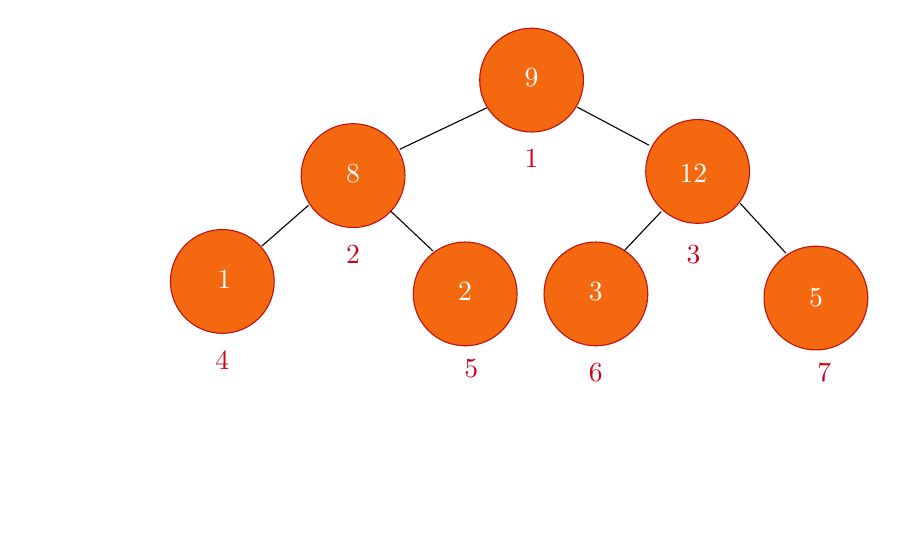
\begin{tikzpicture}[x=0.75pt,y=0.75pt,yscale=-1,xscale=1]
    	%uncomment if require: \path (0,300); %set diagram left start at 0, and has height of 300
    	
    	\draw  [color={rgb, 255:red, 189; green, 19; blue, 19 }  ,draw opacity=1 ][fill={rgb, 255:red, 244; green, 105; blue, 16 }  ,fill opacity=1 ]  (321, 32) circle [x radius= 25, y radius= 25]  ;
    	\draw  [color={rgb, 255:red, 189; green, 19; blue, 19 }  ,draw opacity=1 ][fill={rgb, 255:red, 244; green, 105; blue, 16 }  ,fill opacity=1 ]  (235, 78) circle [x radius= 25, y radius= 25]  ;
    	\draw    (257.5,65.33) -- (299.5,45.33) ;
    	
    	
    	\draw  [color={rgb, 255:red, 189; green, 19; blue, 19 }  ,draw opacity=1 ][fill={rgb, 255:red, 244; green, 105; blue, 16 }  ,fill opacity=1 ]  (401, 76) circle [x radius= 25, y radius= 25]  ;
    	\draw    (343,45) -- (377.5,63.33) ;
    	
    	
    	\draw  [color={rgb, 255:red, 189; green, 19; blue, 19 }  ,draw opacity=1 ][fill={rgb, 255:red, 244; green, 105; blue, 16 }  ,fill opacity=1 ]  (172, 129) circle [x radius= 25, y radius= 25]  ;
    	\draw    (191,112) -- (213.5,92.33) ;
    	
    	
    	\draw  [color={rgb, 255:red, 189; green, 19; blue, 19 }  ,draw opacity=1 ][fill={rgb, 255:red, 244; green, 105; blue, 16 }  ,fill opacity=1 ]  (289, 135) circle [x radius= 25, y radius= 25]  ;
    	\draw    (253,95) -- (273.5,114.33) ;
    	
    	
    	\draw  [color={rgb, 255:red, 189; green, 19; blue, 19 }  ,draw opacity=1 ][fill={rgb, 255:red, 244; green, 105; blue, 16 }  ,fill opacity=1 ]  (352, 135) circle [x radius= 25, y radius= 25]  ;
    	\draw    (365.5,114.33) -- (383.5,95.33) ;
    	
    	
    	\draw  [color={rgb, 255:red, 189; green, 19; blue, 19 }  ,draw opacity=1 ][fill={rgb, 255:red, 244; green, 105; blue, 16 }  ,fill opacity=1 ]  (458, 137) circle [x radius= 25, y radius= 25]  ;
    	\draw    (421.5,91.33) -- (443.5,115.33) ;
    	
    	
    	
    	\draw (321,31) node [color={rgb, 255:red, 255; green, 255; blue, 255 }  ,opacity=1 ] [align=left] {9};
    	\draw (321,70) node [color={rgb, 255:red, 208; green, 2; blue, 27 }  ,opacity=1 ] [align=left] {1};
    	\draw (235,77) node [color={rgb, 255:red, 255; green, 255; blue, 255 }  ,opacity=1 ] [align=left] {8};
    	\draw (235,116) node [color={rgb, 255:red, 208; green, 2; blue, 27 }  ,opacity=1 ] [align=left] {2};
    	\draw (399,77) node [color={rgb, 255:red, 255; green, 255; blue, 255 }  ,opacity=1 ] [align=left] {12};
    	\draw (399,116) node [color={rgb, 255:red, 208; green, 2; blue, 27 }  ,opacity=1 ] [align=left] {3};
    	\draw (173,128) node [color={rgb, 255:red, 255; green, 255; blue, 255 }  ,opacity=1 ] [align=left] {1};
    	\draw (172,167) node [color={rgb, 255:red, 208; green, 2; blue, 27 }  ,opacity=1 ] [align=left] {4};
    	\draw (86,174) node [color={rgb, 255:red, 255; green, 255; blue, 255 }  ,opacity=1 ] [align=left] {1};
    	\draw (250,174) node [color={rgb, 255:red, 255; green, 255; blue, 255 }  ,opacity=1 ] [align=left] {5};
    	\draw (289,134) node [color={rgb, 255:red, 255; green, 255; blue, 255 }  ,opacity=1 ] [align=left] {2};
    	\draw (292,171) node [color={rgb, 255:red, 208; green, 2; blue, 27 }  ,opacity=1 ] [align=left] {5};
    	\draw (352,134) node [color={rgb, 255:red, 255; green, 255; blue, 255 }  ,opacity=1 ] [align=left] {3};
    	\draw (352,173) node [color={rgb, 255:red, 208; green, 2; blue, 27 }  ,opacity=1 ] [align=left] {6};
    	\draw (290,185) node [color={rgb, 255:red, 255; green, 255; blue, 255 }  ,opacity=1 ] [align=left] {1};
    	\draw (367,231) node [color={rgb, 255:red, 255; green, 255; blue, 255 }  ,opacity=1 ] [align=left] {5};
    	\draw (458,137) node [color={rgb, 255:red, 255; green, 255; blue, 255 }  ,opacity=1 ] [align=left] {5};
    	\draw (462,173) node [color={rgb, 255:red, 208; green, 2; blue, 27 }  ,opacity=1 ] [align=left] {7};
    	
    	
    	\end{tikzpicture}
    \end{center}
\end{frame}


\begin{frame}
	\begin{center}
		\tikzset{every picture/.style={line width=0.75pt}} %set default line width to 0.75pt        
		
		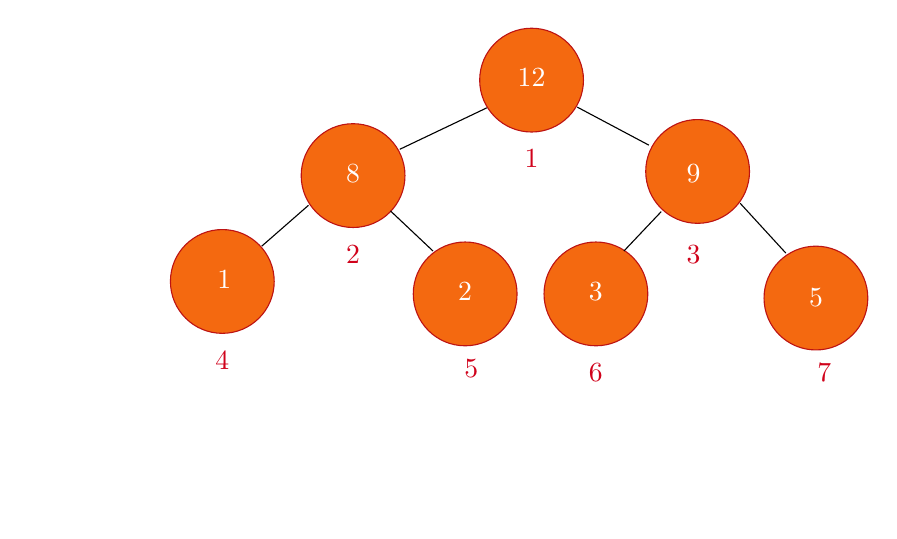
\begin{tikzpicture}[x=0.75pt,y=0.75pt,yscale=-1,xscale=1]
		%uncomment if require: \path (0,300); %set diagram left start at 0, and has height of 300
		
		\draw  [color={rgb, 255:red, 189; green, 19; blue, 19 }  ,draw opacity=1 ][fill={rgb, 255:red, 244; green, 105; blue, 16 }  ,fill opacity=1 ]  (321, 32) circle [x radius= 25, y radius= 25]  ;
		\draw  [color={rgb, 255:red, 189; green, 19; blue, 19 }  ,draw opacity=1 ][fill={rgb, 255:red, 244; green, 105; blue, 16 }  ,fill opacity=1 ]  (235, 78) circle [x radius= 25, y radius= 25]  ;
		\draw    (257.5,65.33) -- (299.5,45.33) ;
		
		
		\draw  [color={rgb, 255:red, 189; green, 19; blue, 19 }  ,draw opacity=1 ][fill={rgb, 255:red, 244; green, 105; blue, 16 }  ,fill opacity=1 ]  (401, 76) circle [x radius= 25, y radius= 25]  ;
		\draw    (343,45) -- (377.5,63.33) ;
		
		
		\draw  [color={rgb, 255:red, 189; green, 19; blue, 19 }  ,draw opacity=1 ][fill={rgb, 255:red, 244; green, 105; blue, 16 }  ,fill opacity=1 ]  (172, 129) circle [x radius= 25, y radius= 25]  ;
		\draw    (191,112) -- (213.5,92.33) ;
		
		
		\draw  [color={rgb, 255:red, 189; green, 19; blue, 19 }  ,draw opacity=1 ][fill={rgb, 255:red, 244; green, 105; blue, 16 }  ,fill opacity=1 ]  (289, 135) circle [x radius= 25, y radius= 25]  ;
		\draw    (253,95) -- (273.5,114.33) ;
		
		
		\draw  [color={rgb, 255:red, 189; green, 19; blue, 19 }  ,draw opacity=1 ][fill={rgb, 255:red, 244; green, 105; blue, 16 }  ,fill opacity=1 ]  (352, 135) circle [x radius= 25, y radius= 25]  ;
		\draw    (365.5,114.33) -- (383.5,95.33) ;
		
		
		\draw  [color={rgb, 255:red, 189; green, 19; blue, 19 }  ,draw opacity=1 ][fill={rgb, 255:red, 244; green, 105; blue, 16 }  ,fill opacity=1 ]  (458, 137) circle [x radius= 25, y radius= 25]  ;
		\draw    (421.5,91.33) -- (443.5,115.33) ;
		
		
		
		\draw (321,31) node [color={rgb, 255:red, 255; green, 255; blue, 255 }  ,opacity=1 ] [align=left] {12};
		\draw (321,70) node [color={rgb, 255:red, 208; green, 2; blue, 27 }  ,opacity=1 ] [align=left] {1};
		\draw (235,77) node [color={rgb, 255:red, 255; green, 255; blue, 255 }  ,opacity=1 ] [align=left] {8};
		\draw (235,116) node [color={rgb, 255:red, 208; green, 2; blue, 27 }  ,opacity=1 ] [align=left] {2};
		\draw (399,77) node [color={rgb, 255:red, 255; green, 255; blue, 255 }  ,opacity=1 ] [align=left] {9};
		\draw (399,116) node [color={rgb, 255:red, 208; green, 2; blue, 27 }  ,opacity=1 ] [align=left] {3};
		\draw (173,128) node [color={rgb, 255:red, 255; green, 255; blue, 255 }  ,opacity=1 ] [align=left] {1};
		\draw (172,167) node [color={rgb, 255:red, 208; green, 2; blue, 27 }  ,opacity=1 ] [align=left] {4};
		\draw (86,174) node [color={rgb, 255:red, 255; green, 255; blue, 255 }  ,opacity=1 ] [align=left] {1};
		\draw (250,174) node [color={rgb, 255:red, 255; green, 255; blue, 255 }  ,opacity=1 ] [align=left] {5};
		\draw (289,134) node [color={rgb, 255:red, 255; green, 255; blue, 255 }  ,opacity=1 ] [align=left] {2};
		\draw (292,171) node [color={rgb, 255:red, 208; green, 2; blue, 27 }  ,opacity=1 ] [align=left] {5};
		\draw (352,134) node [color={rgb, 255:red, 255; green, 255; blue, 255 }  ,opacity=1 ] [align=left] {3};
		\draw (352,173) node [color={rgb, 255:red, 208; green, 2; blue, 27 }  ,opacity=1 ] [align=left] {6};
		\draw (290,185) node [color={rgb, 255:red, 255; green, 255; blue, 255 }  ,opacity=1 ] [align=left] {1};
		\draw (367,231) node [color={rgb, 255:red, 255; green, 255; blue, 255 }  ,opacity=1 ] [align=left] {5};
		\draw (458,137) node [color={rgb, 255:red, 255; green, 255; blue, 255 }  ,opacity=1 ] [align=left] {5};
		\draw (462,173) node [color={rgb, 255:red, 208; green, 2; blue, 27 }  ,opacity=1 ] [align=left] {7};
		
		
		\end{tikzpicture}
	\end{center}
\end{frame}





   
\end{document}

















